\chapter{Recuperação da Informação}
\label{cap:informationretrieval}

\begin{quotation}[]{Yoko Ono}
The computer is my favourite invention. I feel lucky to be part of the global village. I don't mean to brag, but I'm so fast with technology. People think it all seems too much, but we'll get used to it. I'm sure it all seemed too much when we were learning to walk.
\end{quotation}

Conforme foi descrito no capítulo \ref{cap:introduction}, na WEB 3.0, o volume de informações cada vez maior tornou necessária a existência de meios para encontrar a informação. O conteúdo, atualmente, não é feito só pra a compreensão humana, mas também para a compreensão das máquinas. Os usuários exigem que as informações desejadas sejam disponibilizadas quase que imediatamente e com precisão. Neste capítulo será abordado tópico de \ac{RI}, onde serão vistos as diferenças entre este e \ac{RD}, além das técnicas mais comumente utilizadas para realizar suas taregas.

\section{Introdução}
Recuperar informações é um processo que pode ser bastante impreciso, é exigido de uma máquina uma capacidade quase humana, a da interpretação. Por conta disso, muitas vezes se é esperado do usuário a capacidade de saber explicar corretamente para uma máquina os seus anseios, já não existe nenhuma tecnologia capaz de interpretar exatamente o pensamento humano nem de compreender por completo a relevância dos resultados que podem ser trazidos. o que normalmente se faz é buscar extrair o máximo de informação possível da expressão feita pelo usuário, através de técnicas de \ac{NLP} como será visto mais adiante.

Além disso, há um requisito de tempo, todo o processo de interpretação das buscas e recuperação dos resultados, deve ser feito quase que instantaneamente. Tendo isso em mente, a indexação é uma das principais técnicas utilizadas para facilitar a recuperação e o cálculo de relevância de vários algoritmos \cite{Fred2008}. Não somente isso, mas técnicas para divisão da carga de trabalho tornaram-se mais comuns pra lidar com tamanha celeridade dos dados.

\section{Recuperação de Informação versus Recuperação de Dados}
Recuperação de Informação pode ser facilmente confundida com outros meios de acesso à informação. Ao contrário de sistemas baseados em conhecimento, sistemas de recuperação de informação não realizam conclusões a partir dos documentos acessados. Os sistemas baseados em conhecimento dependem de uma visão de mundo pré-definida para poder realizar inferências e gerar informação, muitas vezes o limitando. Já o propósito geral da recuperação de informação é conseguir entregar ao usuário documentos que possam satisfazer sua necessidade de informação \citep{Ruthven2003}, permitindo uma visão mais ampla.

A recuperação da informação permite que existam diferenças entre o que foi requisitado pelo usuário e o que foi apresentado como resultado, desde que haja uma similaridade. A Recuperação de Dados (\ac{RD}), por outro lado, tenta garantir que a consulta irá trazer apenas o que foi especificado na consulta. Por conta disso, embora a recuperação da informação esteja sujeita à imprecisão e possíveis erros, a mesma é capaz de abranger um conteúdo maior e trazer resultados relacionados que não dependam tanto da capacidade do usuário de gerar uma consulta adequada, enquanto que a recuperação de dados, exige que o usuário tenha a capacidade de expressar perfeitamente sua necessidade e tem uma falha total quando não o consegue. Este mérito deve-se a capacidade de lidar com textos semi-estruturados de linguagem natural, enquanto que a recuperação de dados, acessa um ambiente, que embora seja estruturado, é limitado, um banco de dados relacional, por exemplo \cite{Fred2008}.

\begin{table}[htb]
	\centering
	\caption{Diferença entre sistemas \ac{RI} e \ac{RD}.}
	\label{tab:RIxRD}
	\begin{tabular}{|m{7cm} | m{2cm} | m{2cm} |}

		\hline
		
		\multicolumn{1}{|c|}{\bfseries Características / Métodos } & \multicolumn{1}{c|}{\bfseries RI} & \multicolumn{1}{c|}{\bfseries RD}\\ \hline
		Combinação exata   					&		&	x 	\\ \hline
		Alta sensibilidade a erros   			&		&	x  	\\ \hline
		Tratamento semântico   				&	x 	&	 	\\ \hline
		Busca em dados não estruturados   	&	x 	&	 	\\ \hline
		Inferência Dedutiva  					&		&	x  	\\ \hline
		Inferência Indutiva   					&	x 	&	 	\\ \hline
		Consulta de sintaxe controlada   		&		&	x 	\\ \hline
		Consulta com linguagem Natural   	&	x 	&	 	\\ \hline
		Mais utilizado em meios acadêmicos   &	x 	&	 	\\ \hline
		Comum em Produtos Comerciais   	&		&	x 	\\ \hline
		
	\end{tabular}
\end{table}
%TODO Referência na tabela?

Seus casos de uso diferem, para este projeto, onde a maior parte do conteúdo é textual e desestruturado, é exatamente onde se encontra a informação desejada. Ainda de acordo com \cite{Fred2008}, as pessoas que usam sistemas de recuperação de informação procuram muito mais além do que apenas aquela exata combinação de palavras, inclusive, muito frequentemente o autor da consulta não detém informação suficiente sobre o domínio da sua busca para realizar buscas mais exatas. Sua consulta serve para encontrar um espaço mais amplo de respostas onde suas palavras-chave estão inseridas, ou talvez ainda, sinônimos ou referências similares, ainda que não sejam idênticos ao que foi especificado. Entretanto, mais comumente, são usados sistemas com recuperação de dados, onde informações relacionadas não são capazes de resolver o problema de um usuário. Aplicações com funcionalidades de cadastro, acesso à bancos, operações administrativas e outros, são muito comuns e não fariam sentido ao recuperar informações senão as exatamente definidas pelo usuário. 

\section{Processamento de linguagem natural}
\subsection{Histórico}
Teste de Turing
\subsection{Análise de documentos}
Cada tópico passará por transformações antes de serem armazenadas. Considere os títulos descritas na tabela \ref{tab:example} no seu estado inicial. Estes irão ilustrar o pré-processamento. Vale ressaltar que o mesmo processo que está sendo descrito com os títulos também ocorre com o corpo.

\begin{table}[htb]
	\centering
    \def\arraystretch{1.2} % padding da linhas da tabela
    \begin{tabular}{|l|l|}
        \hline
        1 & <p>I will organize this room</p>            \\ \hline
        2 & All rooms are organized and clean \\ \hline
        3 & Cleaners are <b>very</b> effective                              \\ \hline
        4 & I will open this window                            \\ \hline
    \end{tabular}
	\caption{Frases de exemplo}
    \label{tab:example}
\end{table}


\subsection{Filtros de caracteres}
Na web é comum encontrar documentos com tags HTML. Para este projeto, estas tags não terão importância, portanto serão removidas e apenas será deixado apenas o texto. É possível verificar o resultado exemplificado na tabela \ref{tab:charfilter}.

\begin{table}[htb]
	\centering
    \def\arraystretch{1.2} % padding da linhas da tabela
    \begin{tabular}{|l|l|l|}
        \hline
        & \textbf{Antes} & \textbf{Depois} \\ \hline
        1 & <p>I will organize this room</p> & I will organize this room            \\ \hline
        2 & All rooms are organized and clean & All rooms are organized and clean \\ \hline
        3 & Cleaners are <b>very</b> effective & Cleaners are very effective                              \\ \hline
        4 & I will open this window & I will open this window                             \\ \hline
    \end{tabular}
	\caption{Frases de exemplo após os filtros de caracteres}
    \label{tab:charfilter}
\end{table}

\subsection{Tokenização}
O processo de tokenização é responsável por dividir um texto em unidades menores. Essas unidades podem ser palavras, caracteres, cadeia de palavras ou cadeia de caracteres. 

Para este projeto, foi usado a tokenização dividindo o conteúdo do texto em palavras usando o algoritmo Unicode Text Segmentation \cite{unicodesegmentation}.

\begin{table}[htb]
	\centering
    \def\arraystretch{1.2} % padding da linhas da tabela
    \begin{tabular}{|l|l|l|}
        \hline
        & \textbf{Antes} & \textbf{Depois} \\ \hline
        1 & I will organize this room & [I, will, organize, this, room]            \\ \hline
        2 & All rooms are organized and clean & [All, rooms, are, organized, and, clean] \\ \hline
        3 & Cleaners are very effective & [Cleaners, are, very, effective]                              \\ \hline
        4 & I will open this window & [I, will, open, this, window]                             \\ \hline
    \end{tabular}
	\caption{Frases de exemplo após a tokenização}
    \label{tab:tokenization}
\end{table}

\subsection{Filtros de tokens}
\subsubsection{Uniformização}
 Foi usada nesse projeto uma transformação responsável por deixar todos os caracteres minúsculos.

\begin{table}[htb]
	\centering
    \def\arraystretch{1.2} % padding da linhas da tabela
    \begin{tabular}{|l|l|l|}
        \hline
        & \textbf{Antes} & \textbf{Depois} \\ \hline
        1 & [I, will, organize, this, room] & [i, will, organize, this, room]            \\ \hline
        2 & [All, rooms, are, organized, and, clean] & [all, rooms, are, organized, and, clean] \\ \hline
        3 & [Cleaners, are, very, effective] & [cleaners, are, very, effective]                              \\ \hline
        4 & [I, will, open, this, window] & [i, will, open, this, window]                             \\ \hline
    \end{tabular}
	\caption{Frases de exemplo após as transformações}
    \label{tab:transformations}
\end{table}

\subsubsection{Remoção de Stop Words}
Existem palavras que adicionam pouco valor semântico ao texto, são conhecidas como \textit{stop words}. Stop words são palavras como: isso, um, a, o, que. Estas também serão removidas. Existem diversas formas de as detectar em um corpus, as mais comuns são com uso de listas com stop words predefinidas ou definindo um limiar máximo de ocorrências que uma palavra pode ter. Assume-se que palavras que ocorrem frequentemente em vários documentos não agregam muito conteúdo ao texto.

\begin{table}[htb]
	\centering
    \def\arraystretch{1.2} % padding da linhas da tabela
    \begin{tabular}{|l|l|l|}
        \hline
        & \textbf{Antes} & \textbf{Depois} \\ \hline
        1 & [i, will, organize, this, room] & [organize, room]            \\ \hline
        2 & [all, rooms, are, organized, and, clean] & [rooms, organized, clean] \\ \hline
        3 & [cleaners, are, very, effective] & [cleaners, effective]                              \\ \hline
        4 & [i, will, open, this, window] & [open, window]                             \\ \hline
    \end{tabular}
	\caption{Frases de exemplo após a remoção de stop words}
    \label{tab:tokenfilter}
\end{table}

\subsubsection{Stemming}
O propósito do stemming é reduzir a variação morfológica das palavras \cite{stemmingdef}. Documentos podem usar formas diferentes de uma palavra, por exemplo, um deles pode usar organizar, outro pode usar organizando e outro organizado. Embora as palavras não sejam idênticas, elas trazem consigo um sentido similar, o que pode ser útil em um sistema de recuperação da informação onde se deseja conteúdo relacionado, ainda que não idêntico.

\begin{figure}[htb]
	\centering
	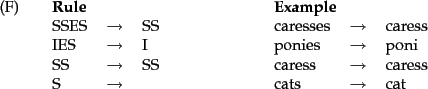
\includegraphics[width=\textwidth]{chapters/project/porterrules.png}
	\caption{Regras usadas na primeira fase do Porter Stemmer}
    \label{fig:porterstemmerprocess}
\end{figure}

O algoritmo mais comum de Stemming é o Porter \cite{porterstemming}. Este algoritmo usa fases com conjuntos definidos de regras para definir as transformações que uma dada palavra irá passar. A figura \ref{fig:porterstemmerprocess} mostra algumas das regras executadas na primeira fase do algoritmo.

Pode-se ver que agora, que as frases descritas na tabela \ref{tab:tokenfilter}, possuem mais palavras em comum do que anteriormente, isso garante uma busca mais abrangente, permitindo o usuário ter resultados com palavras diferentes da sua, mas que ainda acessem o mesmo domínio. Entretanto o resultado não é perfeito, palavras relacionadas podem acabar tendo finais diferentes e palavras diferentes podem possuir o mesmo resultado.
\begin{table}[htb]
	\centering
    \def\arraystretch{1.2}
    \begin{tabular}{|l|l|l|}
        \hline
        & \textbf{Antes} & \textbf{Depois} \\ \hline
        1 & [organize, room]  & [organ, room]            \\ \hline
        2 & [rooms, organized, clean]  & [room, organ, clean] \\ \hline
        3 & [cleaners, effective]  & [cleaner, effect]                              \\ \hline
        4 & [open, window]  & [open, window]                             \\ \hline
    \end{tabular}
	\caption{Frases de exemplo após o stemming}
    \label{tab:tokenfilter}
\end{table}

\subsection{Aplicações}
\begin{itemize}
    \item Sumarização de textos
    \item Question Answering
    \item Análise de sentimento
    \item Assistentes pessoais
    \item Tradução
\end{itemize}

\section{Estratégias de Recuperação}

De acordo com \citep{Grossman2004}, as estratégias de recuperação atribuem uma medida de similaridade entre uma consulta e um documento. Essas estratégias são baseadas na quantidade de ocorrências do termo em um documento. Quanto mais frequente o termo, mais relevante o documento. Além disso algumas dessas estratégias tratam das ambiguidades dos termos, e.g, \textit{rio de janeiro} e \textit{cidade maravilhosa}, podem ser referência ao mesmo conceito.
Os algoritmos consistem de uma consulta \textit{c} e um conjunto de documentos \textit{d\textsubscript{1}}, \textit{d\textsubscript{2}}, ..., \textit{d\textsubscript{n}} o coeficiente de similaridade é dado por \textit{SC(c,d\textsubscript{i})} para \textit{1 <= i <= n}.



\section{Modelo Probabilístico de Recuperação}

Como brevemente abordado na seção anterior, o modelo de espaço vetorial calcula a medida de similaridade através da definição de vetores. O conteúdo de cada documento e os termos da consulta, conforme ilustrado na Figura \ref{fig:documento-vetor}, são traduzidos em vetores e dessa forma é possível medir a similaridade através de operações feitas em cima desses vetores. Os documentos cujo conteúdo, conforme medido através dos termos presentes no documento, correspondem mais ao conteúdo da consulta, são considerados os mais relevantes \citep{Grossman2004}.

\begin{figure}[htb]
	\centering
	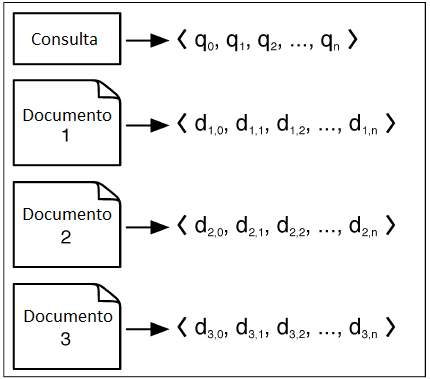
\includegraphics[scale=1.0]{chapters/informationretrieval/Document_as_Vectors.png}
	\caption{Representação dos vetores do modelo de espaço vetorial \citep{Grossman2004}.}
	\label{fig:documento-vetor}
\end{figure}

Este modelo envolve a construção de um vetor que representa os termos de um documento e outro vetor que representa os termos da pesquisa. Em seguida, um método de avaliação deve ser escolhido para medir o grau de aproximação de qualquer vetor documento com o vetor da consulta. Pode-se avaliar a diferença entre a magnitude entre dois vetores, mas geralmente isso prejudica documentos muito grandes e pode dar vantagem para documentos pequenos mas que não possuem muita similaridade \citep{Croft2010}.

Para continuar o entendimento sobre a similaridade desse modelo, é importante alguns conceitos sobre frequência de termos, frequência em documentos e frequência em coleção de documentos que serão abordados em seguida.

\subsection{Frequência de Termos}

De acordo com \cite{Manning2008}, um documento que menciona um termo da consulta mais frequentemente, pode ter uma relação maior com a consulta e, portanto, deveria receber uma pontuação maior. Veremos mais adiante que essa afirmação pode não ser verdade para todos os casos.

Tratando-se de frequência de termos bruta, atribuímos a cada termo de um documento um peso que depende do número de ocorrências do termo no documento. Gostaríamos calcular uma pontuação entre um termo da consulta \textit{t} e um documento \textit{d}, com base no peso de \textit{t} em \textit{d}. A abordagem mais simples é atribuir o peso igual ao número de ocorrências de um termo t num documento d. Este esquema de ponderação é referido como Frequência de Termos e é denotado por \textit{tf\textsubscript{t,d}} \citep{Manning2008}.

A ordem no qual os termos aparecem nos documentos não são levadas em consideração. O importante é apenas reter a frequência total dos termos da busca presentes em cada documento. Essa abordagem é conhecida na literatura como \textit{bag of word} \citep{Croft2010}.

\cite{Manning2008} esclarece ainda, que a frequência bruta não garante que um documento que possua um termo citado 20 vezes é mais relevante do que um documento que possui esse mesmo termo citado dez. Isso porque a relevância não aumenta linearmente proporcional à frequência de termos. Deste modo, frequência de termo logarítmica é mais interessante.

\begin{equation}
w_{t,d} = 
\left\{\begin{matrix}
 &1 +  \log_{10}tf_{t,d},  &se\ tf_{t,d} > 0 \\ 
 &0,  &caso\ contrario 
\end{matrix}\right.
\label{eq:log-tf}
\end{equation}

A tabela seguinte exibe um exemplificação da aplicação da frequência logarítmica de um mesmo termo presente em cinco documentos.

\begin{table}[H]
	\centering
	\caption{Exemplo de aplicação de frequência logarítmica de termos.}
	\label{tab:log-tf-table}
	\def\arraystretch{1.2} % padding da linhas da tabela
	\begin{tabular}{|m{3cm} | m{3cm} | m{3cm} |}

		\hline
		
		\multicolumn{1}{|c|}{\bfseries Documento } & \multicolumn{1}{c|}{\bfseries Frequência} & \multicolumn{1}{c|}{\bfseries Frequência log.}\\ \hline
		d1   					&	0		&	0 	\\ \hline
		d2   					&	1		&	1 	\\ \hline
		d3   					&	2		&	1,3 \\ \hline
		d4   					&	10		&	2	\\ \hline
		d5   					&	1000	&	4 	\\ \hline
		
	\end{tabular}
\end{table}

Como pode ser observado, ainda há importância na quantidade de ocorrência do termo, mas essa frequência não é mais tão determinante na relevância já que a frequência logarítmica aproxima os documentos.

\subsection{Frequência Inversa em Documentos}

 A utilização da frequência inversa em documentos vem da ideia de que termos mais raros são semanticamente mais informativos do que termos comuns. Termos comuns geralmente não possuem o poder de determinar o conteúdo de um documento, mas a presença de um termo raro em um documento aumenta a probabilidade deste documento ser estar fortemente relacionado à ele e, consequentemente, mais relevante para a busca \citep{Manning2008}.

Por exemplo, na área de Ciência da Computação, os termos \textit{código} e \textit{algoritmo} estão muito presentes nos mais diversos tipos de documentos. Se um usuário buscar por \textit{algoritmo de Dijkstra} e o sistema der importância igual aos dois termos e buscar por documentos que possuam apenas o termo \textit{algoritmo}, é improvável que esses documentos satisfaçam o usuário. Neste exemplo, o termo \textit{Dijkstra} tem o valor muito mais determinante na busca do que \textit{algoritmo} e, portanto, deve ter um peso maior na escolha dos documentos.

A definição trazida por \cite{Manning2008} diz que a frequência de documentos \textit{df\textsubscript{t}} corresponde ao total de documentos em uma coleção que contém o termo \textit{t} buscado. Disso, a frequência inversa em documentos, é a medida inversa da informatividade de um termo \textit{t}. Ou seja, quanto menor a frequência de documentos que no qual o termo \textit{t} está presente de uma dada coleção de documentos, mais informativo esses documentos devem ser. Essa fórmula é definida por:

\begin{equation}
idf = \log_{10}(N/df_{t})
\label{eq:idf}
\end{equation}

\subsection{TF–IDF}

Com essas duas medidas definidas acima, Frequência de Termos e Frequência Inversa em Documentos, pode-se aplicar \textit{tf-Idf weight} para determinar a importância do termo presente no documento com relação à coleção total de documentos. Em linhas gerais, tf-idf weight aumenta de acordo com o número de ocorrências de um termo e um documento e também aumenta de acordo com a raridade dos termos presentes no mesmo documento \cite{Manning2008}. 

Tf-idf possui três esquemas mas para simplificação e objetivo deste trabalho, abordaremos apenas a seguinte:
 
\begin{equation}
w_{t,d} = (1 + \log tf_{t,d}) \cdot \log_{10}(N/df_{t})
\label{eq:tf-idf}
\end{equation}

\subsection{Okapi BM25}

\section{Métodos de avaliação}
A partir das opções disponibilizadas para construir sistemas de recuperação da informação, resta buscar meios para os avaliar. Considerando que não existe método perfeito para todos os problemas é necessário se conduzir uma pesquisa para averiguar-se qual a melhor solução para determinado problema. Para fazer isso, determinam-se métricas que irão indicar se há conformidade da solução com o problema.

Uma das formas de se executar um experimento para avaliar o sistema é utilizar um conjunto de buscas e seus resultados esperados. A partir dessas buscas, avaliam-se as condições com que foram apresentados os resultados, levando em consideração desde o tempo que custou para achar essas informações até a quantidade de esforço necessária do usuário para encontrar uma informação relevante dentro do conjunto de resultados. Sendo estas as principais condições:
%As métricas mais relevantes podem variar de problema para problema, já que em alguns podemos ter algumas restrições que outros não possuam, como tempo, por exemplo
\begin{itemize}
    \item \textbf{Cobertura}. Representa o quanto de informações relevantes foram apresentadas como resultados. Considerando que para uma busca X existam 10 resultados relevantes, se apenas 3 foram apresentados para o usuário, temos uma cobertura de 30\%.
    \item \textbf{Ranking}. Métricas que utilizam o rank como parâmetro, avaliam o sistema de acordo com a posição dos itens relevantes nos resultados da busca. Um exemplo deste é o Mean Reciprocal Rank, onde para cada busca, a posição do primeiro documento relevante chamada K é usada pra determinar o Reciprocal Rank que é 1/K, em seguida, deve-se continuar executando mais N buscas onde encontraremos a média desses valores a partir de (1/K1 + 1/K2 + ... )/ N para encontrar o Mean Reciprocal Rank.
    \item \textbf{Precisão}. Informa o quanto de conteúdo relevante existe dentre os documentos apresentados. Por exemplo, se dentre 10 resultados retornados, apenas 2 resultados forem relevantes, temos uma precisão de 20\%.
    \item \textbf{Tempo de resposta}. É o intervalo médio entre o momento da consulta e a apresentação dos resultados.
    \item \textbf{Esforço do usuário}. Representa o esforço despendido pelo usuário para obter resultados em sua busca. Isso pode incluir diversos fatores que variam de acordo com a especificação do problema, sendo exemplos deles: número de linhas lida, número de ações necessárias para executar a busca, número de documentos abertos até encontrar o resultado desejado e outros.
\end{itemize}

\section{Tecnologias e Frameworks}

Para melhor lidar com os desafios de Recuperação da Informação, foram criadas novas tecnologias e frameworks. Essas tecnologias implementam os conceitos aqui utilizados e permitem modificações para que se adaptem melhor ao problema em questão. Os seguintes frameworks são os mais populares.

\begin{itemize}
    \item \textbf{Lucene}. O Apache Lucene é um motor de busca escrito em Java com ferramentas para busca em texto. É uma API open source disponível para download gratuito. Possui uma linguagem própria que permite fazer buscas parametrizadas com expressões regulares. 
    \item \textbf{Solr}. Solr é uma aplicação web construída ao redor do Lucene que adiciona funcionalidades como: busca geospacial, replicação, cacheamento e interfaces de administração.
    \item \textbf{Elasticsearch}. Assim como Solr, o Elasticsearch é uma aplicação construída com o uso do Lucene. O Elasticsearch é distribuído pela empresa Elastic e possui diversos plugins gratuitos e pagos para adicionar-se ferramentas de administração. Diferencia-se do Solr por focar mais em aspectos da administração do banco de dados e na escalabilidade.
\end{itemize}

\section{Sumário}

Foi abordado neste capítulo como e onde a Recuperação Informação é utilizada. Foi tratada a diferença entre Recuperação de Informação e Recuperação Dados e abordada algumas estratégias na recuperação de informações e como as avaliar. Houve um aprofundamento em modelos vetoriais, método que será usado neste trabalho.